\subsection{Оцінка орієнтовних значень похибок вимірників первинної інформації БІНС}

Датчики первинної інформації БІНС -- датчики кутової швидкості й акселерометри встановлюються жорстко на ЛА. 
Тяжкі умови роботи датчиків інформації призводять до появи значних похибок, тому в алгоритмах роботи БІНС бажано 
здійснити аналітичну компенсацію похибок вимірників (здійснювати їх польотне калібрування), перш ніж ці сигнали 
будуть використані для розрахунку параметрів орієнтації і для визначення складових уявного прискорення уздовж навігаційних осей.

Інструментальні похибки ІНС визначаються погрішностями аmкселерометрів, вимірників кутової швидкості або кута, 
а також погрішностями обчислювального пристрою. Очевидно, при застосуванні обчислювального пристрою досить високої 
точності похибки, ІНС будуть визначатися головним чином погрішностями первинних вимірювальних датчиків, що входять у систему.

Якщо акселерометри ІНС вимірюють прискорення $a_{x} $ і $a_{y} $ з погрішностями $\Delta a_{x} $ і $\Delta a_{y} $, то,  
це приведе до помилки у визначенні координати $\Delta \lambda _{y} $.

Приладові значення зазначених параметрів (зі значком «*»)

\begin{equation} 
\label{eq:err} 
\left. 
\begin{array}{l} 
{a_{\xi }^{*} =a_{\xi } +\Delta a_{\xi } ;{\rm \; \; }a_{x}^{*} =a_{x} +\Delta a_{x} ;{\rm \; \; \; }a_{y}^{*} =a_{y} +\Delta a_{y} ;} 
\\ {\dot{\lambda }_{y}^{*} =\dot{\lambda }_{y} +\Delta \dot{\lambda }_{y} ;{\rm \; \; \; }\lambda _{y}^{*} =\lambda _{y} 
+\Delta \lambda _{y} ;}
\\ {\ddot{\vartheta }'^{*} =\ddot{\vartheta }'+\Delta \ddot{\vartheta }'; \dot{\vartheta }'^{*} =\dot{\vartheta }'+\Delta \dot{\vartheta }';
{\rm \; \; \; }\vartheta '^{*} =\vartheta '+\Delta \vartheta '.} \end{array}\right\} 
\end{equation} 

Підставивши значення цих параметрів у перші рівняння систем і зробивши відповідні перетворення наступне рівняння похибок:

\begin{equation} 
\label{eq:lam_err} 
\Delta \ddot{\lambda }_{y} +\frac{(a_{\eta } +g_{0} )}{R_{{\text{З}}} } 
\Delta \lambda _{y} =\frac{1}{R_{{\text{З}}} } \left[a_{x} \cos (\lambda _{y} -\vartheta ')+a_{y} \sin (\lambda _{y} -
\vartheta ')\right] 
\end{equation} 

Як видно, ліва частина рівняння \eqref{eq:lam_err} є (при $a_{\eta } =0$) рівнянням маятника Шулера, а права -- збурюючим впливом.

Координата $\lambda _{y} $ і кут $\vartheta '$ у процесі руху безупинно змінюються, тому права частина рівняння \eqref{eq:lam_err} 
буде теж змінною в часі.

З огляду на вираз і те, що при автоматичному керуванні рухом кут відхилення об'єкта від площини горизонту досить малий, а також вважаючи

\[\Delta a_{x} =\Delta a_{y} =\Delta a\] 

у першому наближенні одержимо

\begin{equation} 
\label{eq:ddot_lambda_1} 
\Delta \ddot{\lambda }_{y} +\frac{1}{R_{{\text{З}}} } (a_{\eta } +g_{0} )\Delta \lambda _{y} \cong \frac{\Delta a}{R_{{\text{З}}} }  
\end{equation} 

При $a_{\eta } =0$, $\Delta a={\rm const}$ рішення рівняння \eqref{eq:ddot_lambda_1} буде наступним:

\begin{equation} 
\label{eq:ddot_lambda_2} 
\Delta \lambda _{y} \cong \frac{\Delta a}{g_{0} } \left(1-\cos \left(\sqrt{\frac{g_{0} }{R_{{\text{З}}} } } \cdot t\right)\right) 
\end{equation} 

З виразу \eqref{eq:ddot_lambda_2} видно, що помилка ІНС у визначенні; координати $\lambda _{y} $, обумовлена похибкою акселерометрів, 
буде мати як постійну, так і змінну складові.Найбільше значення похибки не перевищить  $\Delta \lambda _{y} \le 2\frac{\Delta a}{g_{0} } $. 

%Графік залежності $\Delta \lambda \left(t\right)$, отриманий шляхом моделювання однокомпонентної БІНС, при наявності 
%постійних похибок акселерометрів представлений на мал. 2.5, \textit{а}. 

%\includegraphics[bb=0mm 0mm 208mm 296mm, width=86.2mm, height=65.5mm, viewport=3mm 4mm 205mm 292mm]{image1.ps}\includegraphics[bb=0mm 0mm 208mm 296mm, width=84.4mm, height=65.3mm, viewport=3mm 4mm 205mm 292mm]{image2.ps}                   \textit{а)}                                                                          \textit{б)}


\textbf{Оцінка помилки акселерометрів}

За допомогою \eqref{eq:ddot_lambda_2} можуть бути отримані орієнтовані формули для розрахунку точнісних вимог пропонованих до датчиків первинної 
інформації -- акселерометрам.

\begin{equation} 
\label{eq:acc_err} 
\Delta a\cong \frac{\Delta \lambda _{y} g_{0} }{\left(1-\cos \left(\sqrt{\frac{g_{0} }{R_{{\text{З}}} } } \cdot t\right)\right)}.    
\end{equation} 

Як випливає з \eqref{eq:acc_err} вимоги до точнісних характеристик акселерометрів залежать від проміжків часу 
автономної роботи БІНС у складі комплексної інерціально-супутникової системи навігації. Виходячи з вимог до 
точності визначення координат (СКВ  5 м) отримані орієнтовані значення похибок акселерометра, у залежності 
від очікуваних перерв у роботі супутникової системи навігації. Розрахункові значення точнісних вимоги 
пропонованих до датчиків первинної інформації, зокрема акселерометрів відображені на графіку рис. \ref{fig:acc_err} 

\begin{figure}
\centering
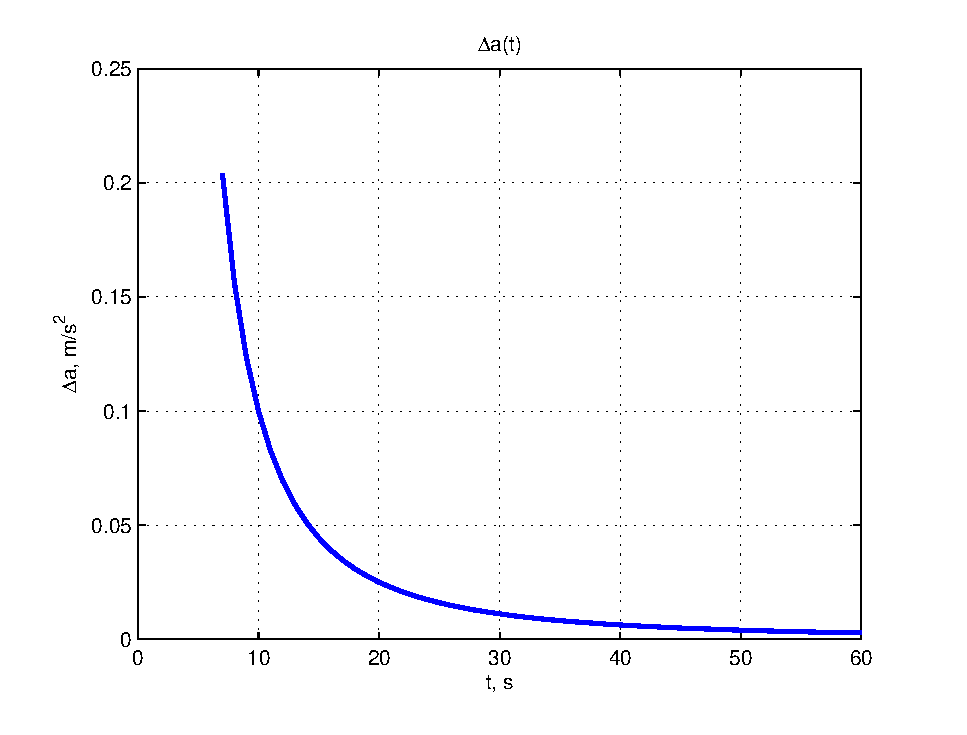
\includegraphics[scale=0.8]{acc_err}
\caption{Графік залежності значень похибок акселерометра від часу}
\label{fig:acc_err}
\end{figure} 
\vline 

\textbf{Оцінка помилки датчика кутової швидкості}

Якщо вимірник кутової швидкості об'єкта має погрішність $\Delta \vartheta '$, то приладове значення кутової швидкості

\[\dot{\vartheta }'^{*} =\dot{\vartheta }'-\Delta \dot{\vartheta }'.\] 

При цьому, будуть мати місце помилки у визначенні інших параметрів.

Підставляючи значення параметрів $\dot{\vartheta }'^{*} $ і  $\lambda _{y}^{*} $ рівняння \eqref{eq:ddot_lambda_1},  
після перетворень з врахуванням другого рівняння системи \eqref{eq:err} одержимо

\begin{equation} 
\label{eq:err_lambda_dot} 
\Delta \ddot{\lambda }_{y} +\frac{a_{\eta } +g_{0} }{R_{\text{З}} } \Delta \lambda _{y} =-\frac{a_{\eta } +g_{0} }{R_{\text{З}} } \Delta \vartheta ' 
\end{equation} 

Як видно ліва частина рівняння \eqref{eq:err_lambda_dot} і в цьому випадку (при $a_{\eta } =0$) представляється рівняння 
маятника Шулера, а права частина -- фактор, що викликається, обумовленими погрішностями у вимірі $\vartheta '$кута .

Якщо вважати погрішність $\Delta \dot{\vartheta }'=\Delta \dot{\vartheta }'_{0} =const$, то $\Delta \vartheta '=\Delta \dot{\vartheta }'_{0} t$, 
при цьому рішення рівняння 
\eqref{eq:err_lambda_dot} буде (якщо $a_{\eta } =0$) наступної:

\begin{equation} 
\label{eq:err_lambda_delta} 
\Delta \lambda _{y} =\Delta \dot{\vartheta }'_{0} \left(\sqrt{\frac{R_{\text{З}} }{g_{0} } } \sin \sqrt{\frac{g_{0} }{R_{\text{З}} } } \cdot t-t\right)
\end{equation} 


Як видно з виразу \eqref{eq:err_lambda_delta},  погрішність у визначенні координати  $\lambda _{y} $, обумовлена 
постійною  помилкою  вимірника кутової швидкості, у першому наближенні має дві складові (рис. 2.5,\textit{б)}, 
одна  з яких  росте пропорційно  часу польоту

\[\Delta \lambda _{y0} =\Delta \dot{\vartheta }'_{0} t,\] 

а інша  змінюється з періодом маятника Шулера

\[\Delta \lambda _{y} =\Delta \dot{\vartheta }'_{0} \sqrt{\frac{R_{\text{З}} }{g_{0} } } \sin \sqrt{\frac{g_{0} }{R_{\text{З}} } } \cdot t\] 


Аналогічно \eqref{eq:acc_err} можуть бути отримані орієнтовані формули для розрахунку точносних вимог 
пропонованих до вимірників кутових швидкостей.

\[\Delta \dot{\vartheta }'_{0} =\frac{\Delta \lambda _{y} }{\left(\sqrt{\frac{R_{{\text{З}}} }{g_{0} } } \sin \left(\sqrt{\frac{g_{0} }{R_{{\text{З}}} } } \cdot t\right)-t\right)} \] 

Виходячи з вимог пропонованих до точносних характеристик визначення координат (СКО $\approx$ 5м) 
отримані орієнтовані значення похибок вимірникам кутових швидкостей, у залежності від очікуваних 
перерв у роботі супутникової системи навігації. Розрахункові значення точнісних вимоги пропонованих 
до датчиків первинної інформації, зокрема вимірникам кутових швидкостей відображені на графіку рис.\ref{fig:gyro_err}.

\begin{figure}[here]
\centering
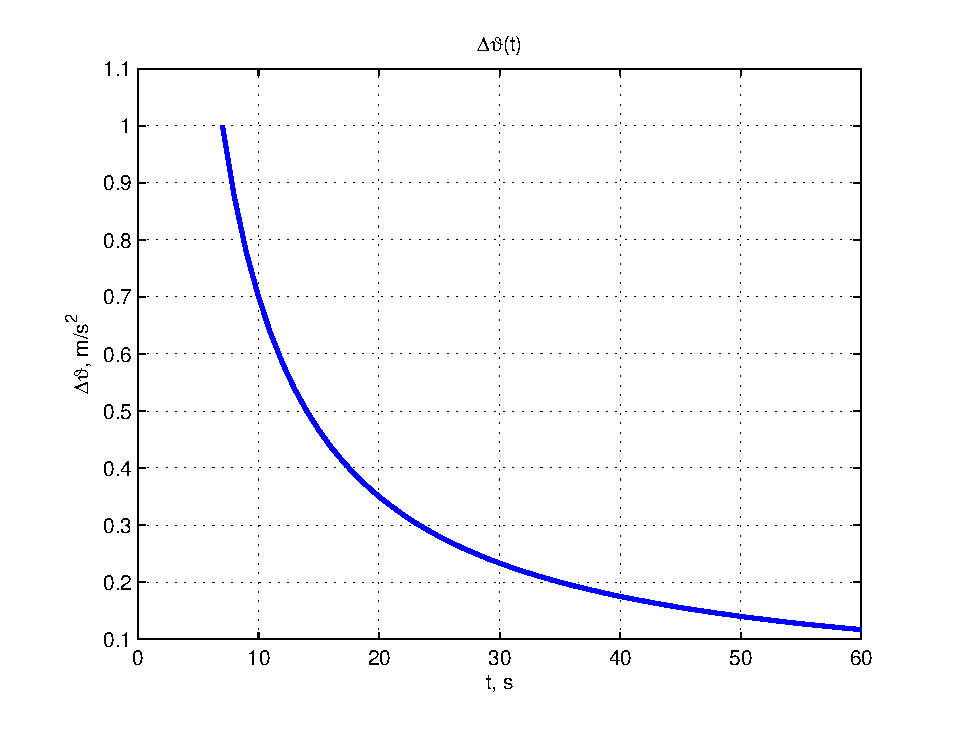
\includegraphics[scale=0.8]{gyro_err}
\caption{Графік залежності значень похибок ДКШ від часу}
\label{fig:gyro_err}
\end{figure} 
% Вихідні похибки БІНС визначаються в основному наступними складовими:
% \begin{enumerate}
%  \item похибками ДКШ і акселерометрів;
%  \item методичними похибками;
%  \item похибками обчислень 
%  \item похибками моделі використовуваної для обліку впливу гравітаційного поля на поводження інерціальних чуттєвих елементів.
% \end{enumerate}
Для БІНС розглянутого класу основний внесок у похибки визначення координат вносять датчики первинної 
інформації. Необхідно відзначити, що методичні похибки, у тому числі похибки, зв'язані зі спрощеннями 
кінематичних рівнянь БІНС, похибками моделювання форми Землі і похибками моделі гравітаційного поля, 
повинні бути не більше  похибок, внесених датчиками первинної інформації.

Багато складові вихідні похибки залежать від параметрів траєкторії й умов роботи, коефіцієнти моделі 
похибок істотно залежать від рівня вібрації і температури. Тому для більш детального дослідження 
точністних характеристик  БІНС необхідна вихідна інформація про аеродинамічні й інерційно масові 
характеристиках літака, а також параметри траєкторії. У цьому випадку можна буде провести детальні 
статистичні дослідження точністних характеристик з урахуванням впливу динамічних похибок датчиків первинної інформації.

Однак при моделюванні враховувалися тільки деякі складові:
\begin{enumerate}
  \item систематичні;
  \item перекручування масштабного коефіцієнта;
  \item випадкові складові;
  \item зони нечутливості
\end{enumerate}

Випадкові складові і перекручування масштабного коефіцієнта моделювалися 
з використанням генераторів "білого шуму" і формуючих фільтрів. При цьому 
вважалося, що кожен чуттєвий елемент цілком визначається значеннями цих 
складових, а самі ці складові змінюються таким чином, що при збільшенні 
одного з них зростають і всі інші. 
\begin{figure}[here]
\centering
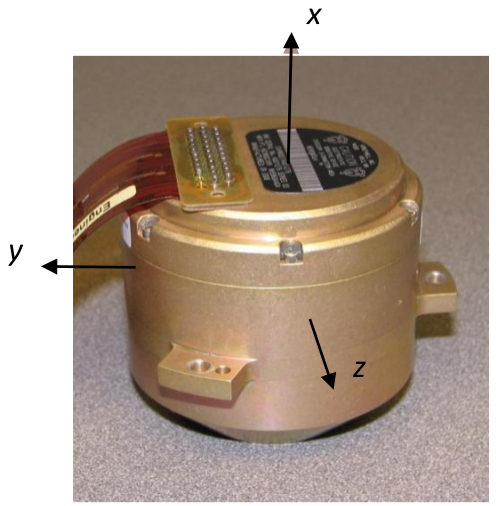
\includegraphics[scale=0.4]{imu_hg1900}
\caption{ДПІ Honeywell HG1900IMU}
\label{fig:imu_hg1900}
\end{figure} 
В роботі пропонується датчики первинної інформації компанії \textit{Honeywell HG1900IMU} (рис.\ref{fig:imu_hg1900}),
які базуються на MEMS технологіях. 

Блок має малі розміри та не велике споживання. Порівняно не велику ціна, через
використання MEMS технології. Недорогий та надійний вбудований процесор серії
\textit{ARM7}. Зручний та надійний герметичний корпус. Програмований з можливістю
масштабування послідовний інтерфейс RS422 .
В наступній таблицях наведені основні параметри датчиків.
\begin{table}[here]
\centering
\caption{Параметри акселерометрів}
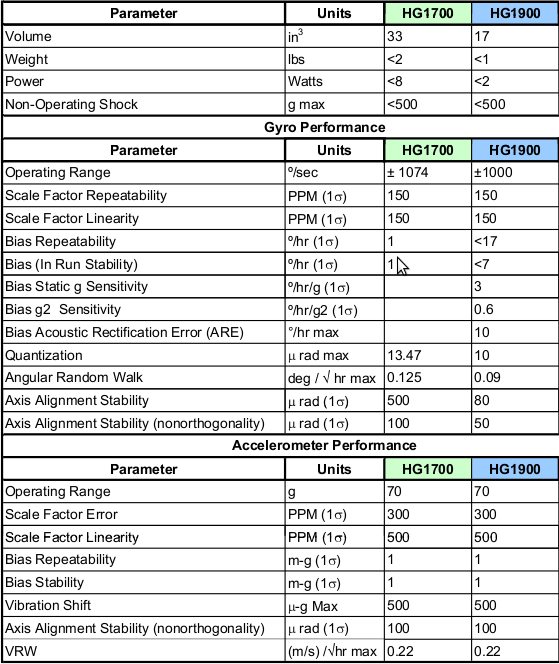
\includegraphics[scale=0.6]{table_hg}

\label{tab:table_hg}
\end{table}










% \begin{table}[here]
% \centering
% \caption{Параметри акселерометрів}
% \begin{tabular}{|p{80mm}|p{20mm}|p{20mm}|p{20mm}|} \hline 
% \multicolumn{4}{|p{1in}|}{Акселерометри} \\ \hline 
% Зсув показань, $10^{-3}$ & 0,01 & 0,05 & 0,1 \\ \hline 
% Масштабний коефіцієнт & 0,001 & 0,005 & 0,01 \\ \hline 
% Неортогональність кут.с & 10 & 10 & 20 \\ \hline 
% Випадкова складова, м/с3/год & 0,009 & 0,01 & 0,02 \\ \hline 
% \end{tabular}
% \label{tab:acc_err}
% \end{table}
% 
% 
% \begin{table}[here]
% \centering
% \caption{Параметри ДКШ}
% 
% \begin{tabular}{|p{80mm}|p{20mm}|p{20mm}|p{20mm}|} \hline
% \multicolumn{4}{|p{1in}|}{ДКШ} \\ \hline 
% Дрейф, що не залежить від перевантаження, град/год & 0,005 & 0,01 & 0,1 \\ \hline 
% Дрейф, що залежить від перевантаження, град/год & 0,0075 & 0,015 & 0,15 \\ \hline 
% Масштабний коефіцієнт & 0,0025 & 0,005 & 0,02 \\ \hline 
% Неортогональність кут.с & 20 & 60 & 120 \\ \hline 
% Випадкове блукання, град/год & 0,0005 & 0,001 & 0,01 \\ \hline 
% \end{tabular}
% \label{tab:gyro_err}
% \end{table}

